%!TeX root=../tese.tex
%("dica" para o editor de texto: este arquivo é parte de um documento maior)
% para saber mais: https://tex.stackexchange.com/q/78101/183146

%% ------------------------------------------------------------------------- %%
\chapter{Algoritmo Guloso}
\label{cap:algoritmo-guloso}

Neste capítulo entenderemos como a visão geométrica de um algoritmo de busca em ABB para uma sequência de acessos $X$ se relaciona com o custo ótimo OPT(X). Além disso, será apresentado um algoritmo guloso offline que transforma um conjunto arboreamente insatisfeito em um conjunto arboreamente satisfeito adicionando uma série de pontos. Por fim, argumentaremos como esse algoritmo offline pode ser adaptado para um algoritmo online em ABBs dentro do modelo de computação adotado.

\section{Otimalidade} 

Revisemos a definição de custo nesse modelo de computação. O custo para realizar um acesso é o número de nós visitados durante esse acesso. Assim, $OPT(X)$ é o menor custo necessário para um algoritmo de busca offline em ABB realizar todos os acessos de uma entrada $X = (x_{1},\ldots,x_{m})$, ou seja, o número mínimo de visitas a nós necessárias para realizar todos os acessos.

Retornando à análise geométrica, seja $P$ um conjunto de pontos, denotaremos por \textit{minASS(P)} o tamanho do menor conjunto arboreamente satisfeito que possui todos os pontos de $P$. 

Seja $P$ a visão geométrica do algoritmo de busca em ABB que possui custo $OPT(X)$ para a sequência de acessos $X$. De acordo com o Lema~\ref{lema:visao_geometrica_vira_ASS}, $P$ é um conjunto arboreamente satisfeito. Além disso, $|P|$ é mínimo para a entrada $X$, pois $P$ é a visão geométrica do algoritmo de busca em ABB que possui o custo ótimo $OPT(X)$. Assim, nota-se que $OPT(X) = minASS(V(X))$, sendo $V(X)$ a visão geométrica da entrada $X$.

Isso implica que o problema de encontrar o custo do algoritmo ótimo de busca em ABBs para uma sequência de acessos $X$ pode ser reformulado como o problema de encontrar o menor superconjunto arboreamente satisfeito da visão geométrica da entrada $X$.

\section{Greedy Future}

%ainda não sabemos porque isso é seção 3 eu acho(?).
%Ainda não se sabe se é possível encontrar o valor de $OPT(X)$ em tempo polinomial, e obviamente pela discussão acima, também não sabemos encontrar o menor superconjunto arboreamente satisfeito, mas apresentaremos um algoritmo guloso chamado Greedy Future que produz um 

Apesar de não se saber se é possível encontrar o valor de $OPT(X)$ em tempo polinomial, e consequentemente encontrar o menor subconjunto arboreamente satisfeito, apresentaremos o algoritmo guloso Greedy Future que dado um conjunto P de pontos que representam uma sequência $X$ de acessos, produz um conjunto de pontos $P'$ que contém P, ou seja, $P' \supseteq P$ e que é arboreamente satisfeito. Estamos assumindo que as sequências de acesso sempre buscam uma única chave em cada instante de tempo, então $P$ obrigatoriamente possui $m$ pontos e todos possuem coordenadas $y$ distintas dentro do intervalo $[1,m]$. 

O algoritmo funciona da seguinte maneira: inicialmente defina uma reta horizontal $r$ em $y = 1$ e inicialize $P' = P$. Seja $a$ um ponto coordenadas $(a.x, a.y)$ e que $a \in P'$ e $a \in r$. Para cada $\{a,b\}$-retângulo insatisfeito com $b.y < a.y$, adicione um ponto em $(b.x, a.y)$. Após satisfazer todos $\{a,b\}$-retângulos, mova $r$ uma unidade para cima e repita. O algoritmo termina após satisfazer todos os $\{a,b\}$-retângulos com $r$ em $y = m$. Veja a Figura~\ref{fig:GreedyFuture-funcionamento}.

\begin{figure}
    \centering
    
    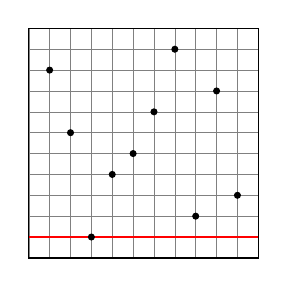
\begin{tikzpicture}[scale=0.265]
        \draw[very thin, gray] (0,0) grid (11,11);
        
        \draw[red, thick] (0,1) -- (11,1);

        \filldraw[black] (3,1) circle (4pt);
        \filldraw[black] (8,2) circle (4pt);
        \filldraw[black] (10,3) circle (4pt);
        \filldraw[black] (4,4) circle (4pt);
        \filldraw[black] (5,5) circle (4pt);
        \filldraw[black] (2,6) circle (4pt);
        \filldraw[black] (6,7) circle (4pt);
        \filldraw[black] (9,8) circle (4pt);
        \filldraw[black] (1,9) circle (4pt);
        \filldraw[black] (7,10) circle (4pt);
        \draw[black, line width=0.5pt] (0,0) rectangle (11,11);
    \end{tikzpicture}
    \hfill 
    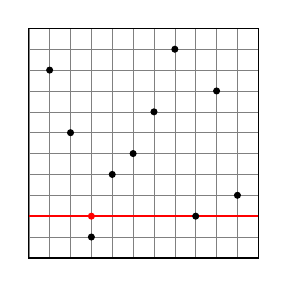
\begin{tikzpicture}[scale=0.265]
        \draw[very thin, gray] (0,0) grid (11,11);
        
        \draw[red, thick] (0,2) -- (11,2);

        \filldraw[black] (3,1) circle (4pt);
        \filldraw[black] (8,2) circle (4pt);
        \filldraw[black] (10,3) circle (4pt);
        \filldraw[black] (4,4) circle (4pt);
        \filldraw[black] (5,5) circle (4pt);
        \filldraw[black] (2,6) circle (4pt);
        \filldraw[black] (6,7) circle (4pt);
        \filldraw[black] (9,8) circle (4pt);
        \filldraw[black] (1,9) circle (4pt);
        \filldraw[black] (7,10) circle (4pt);
        \filldraw[red] (3,2) circle (4pt);

        \draw[black, line width=0.5pt] (0,0) rectangle (11,11);
    \end{tikzpicture}
    \hfill 
    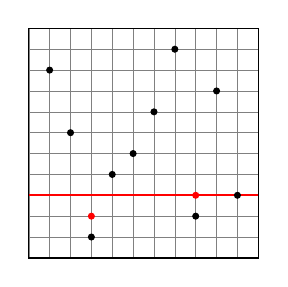
\begin{tikzpicture}[scale=0.265]
        \draw[very thin, gray] (0,0) grid (11,11);
        
        \draw[red, thick] (0,3) -- (11,3);

        \filldraw[black] (3,1) circle (4pt);
        \filldraw[black] (8,2) circle (4pt);
        \filldraw[black] (10,3) circle (4pt);
        \filldraw[black] (4,4) circle (4pt);
        \filldraw[black] (5,5) circle (4pt);
        \filldraw[black] (2,6) circle (4pt);
        \filldraw[black] (6,7) circle (4pt);
        \filldraw[black] (9,8) circle (4pt);
        \filldraw[black] (1,9) circle (4pt);
        \filldraw[black] (7,10) circle (4pt);
        \filldraw[red] (3,2) circle (4pt);
        \filldraw[red] (8,3) circle (4pt);
        \draw[black, line width=0.5pt] (0,0) rectangle (11,11);
    \end{tikzpicture}
    \hfill 
    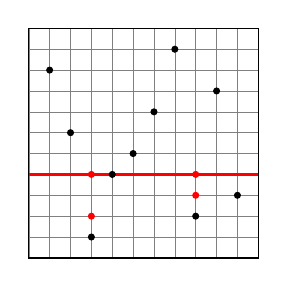
\begin{tikzpicture}[scale=0.265]
        \draw[very thin, gray] (0,0) grid (11,11);
        
        \draw[red, thick] (0,4) -- (11,4);

        \filldraw[black] (3,1) circle (4pt);
        \filldraw[black] (8,2) circle (4pt);
        \filldraw[black] (10,3) circle (4pt);
        \filldraw[black] (4,4) circle (4pt);
        \filldraw[black] (5,5) circle (4pt);
        \filldraw[black] (2,6) circle (4pt);
        \filldraw[black] (6,7) circle (4pt);
        \filldraw[black] (9,8) circle (4pt);
        \filldraw[black] (1,9) circle (4pt);
        \filldraw[black] (7,10) circle (4pt);
        \filldraw[red] (3,2) circle (4pt);
        \filldraw[red] (8,3) circle (4pt);
        \filldraw[red] (3,4) circle (4pt);
        \filldraw[red] (8,4) circle (4pt);
        \draw[black, line width=0.5pt] (0,0) rectangle (11,11); 
    \end{tikzpicture}
    \hfill 
    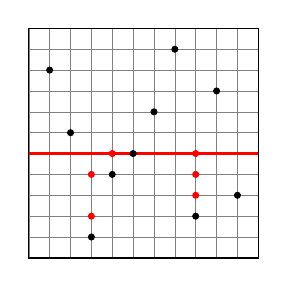
\begin{tikzpicture}[scale=0.265]
        \draw[very thin, gray] (0,0) grid (11,11);
        
        \draw[red, thick] (0,5) -- (11,5);

        \filldraw[black] (3,1) circle (4pt);
        \filldraw[black] (8,2) circle (4pt);
        \filldraw[black] (10,3) circle (4pt);
        \filldraw[black] (4,4) circle (4pt);
        \filldraw[black] (5,5) circle (4pt);
        \filldraw[black] (2,6) circle (4pt);
        \filldraw[black] (6,7) circle (4pt);
        \filldraw[black] (9,8) circle (4pt);
        \filldraw[black] (1,9) circle (4pt);
        \filldraw[black] (7,10) circle (4pt);
        \filldraw[red] (3,2) circle (4pt);
        \filldraw[red] (8,3) circle (4pt);
        \filldraw[red] (3,4) circle (4pt);
        \filldraw[red] (8,4) circle (4pt);
        \filldraw[red] (4,5) circle (4pt);
        \filldraw[red] (8,5) circle (4pt);
        \draw[black, line width=0.5pt] (0,0) rectangle (11,11); 
    \end{tikzpicture}
    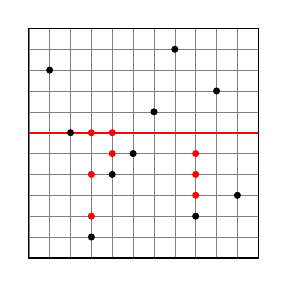
\begin{tikzpicture}[scale=0.265]
        \draw[very thin, gray] (0,0) grid (11,11);
        
        \draw[red, thick] (0,6) -- (11,6);

        \filldraw[black] (3,1) circle (4pt);
        \filldraw[black] (8,2) circle (4pt);
        \filldraw[black] (10,3) circle (4pt);
        \filldraw[black] (4,4) circle (4pt);
        \filldraw[black] (5,5) circle (4pt);
        \filldraw[black] (2,6) circle (4pt);
        \filldraw[black] (6,7) circle (4pt);
        \filldraw[black] (9,8) circle (4pt);
        \filldraw[black] (1,9) circle (4pt);
        \filldraw[black] (7,10) circle (4pt);
        \filldraw[red] (3,2) circle (4pt);
        \filldraw[red] (8,3) circle (4pt);
        \filldraw[red] (3,4) circle (4pt);
        \filldraw[red] (8,4) circle (4pt);
        \filldraw[red] (4,5) circle (4pt);
        \filldraw[red] (8,5) circle (4pt);
        \filldraw[red] (3,6) circle (4pt);
        \filldraw[red] (4,6) circle (4pt);
        \draw[black, line width=0.5pt] (0,0) rectangle (11,11); 
    \end{tikzpicture}
    \hfill 
    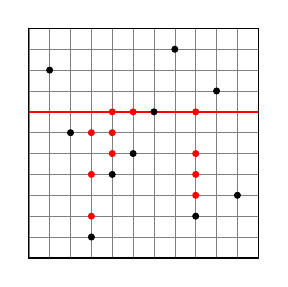
\begin{tikzpicture}[scale=0.265]
        \draw[very thin, gray] (0,0) grid (11,11);
        
        \draw[red, thick] (0,7) -- (11,7);

        \filldraw[black] (3,1) circle (4pt);
        \filldraw[black] (8,2) circle (4pt);
        \filldraw[black] (10,3) circle (4pt);
        \filldraw[black] (4,4) circle (4pt);
        \filldraw[black] (5,5) circle (4pt);
        \filldraw[black] (2,6) circle (4pt);
        \filldraw[black] (6,7) circle (4pt);
        \filldraw[black] (9,8) circle (4pt);
        \filldraw[black] (1,9) circle (4pt);
        \filldraw[black] (7,10) circle (4pt);
        \filldraw[red] (3,2) circle (4pt);
        \filldraw[red] (8,3) circle (4pt);
        \filldraw[red] (3,4) circle (4pt);
        \filldraw[red] (8,4) circle (4pt);
        \filldraw[red] (4,5) circle (4pt);
        \filldraw[red] (8,5) circle (4pt);
        \filldraw[red] (3,6) circle (4pt);
        \filldraw[red] (4,6) circle (4pt);
        \filldraw[red] (4,7) circle (4pt);
        \filldraw[red] (5,7) circle (4pt);
        \filldraw[red] (8,7) circle (4pt);
        \draw[black, line width=0.5pt] (0,0) rectangle (11,11); 
    \end{tikzpicture}
    \hfill 
    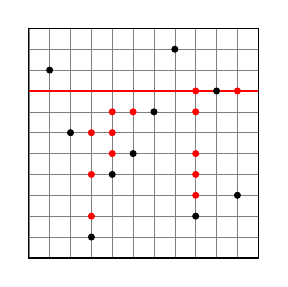
\begin{tikzpicture}[scale=0.265]
        \draw[very thin, gray] (0,0) grid (11,11);
        
        \draw[red, thick] (0,8) -- (11,8);

        \filldraw[black] (3,1) circle (4pt);
        \filldraw[black] (8,2) circle (4pt);
        \filldraw[black] (10,3) circle (4pt);
        \filldraw[black] (4,4) circle (4pt);
        \filldraw[black] (5,5) circle (4pt);
        \filldraw[black] (2,6) circle (4pt);
        \filldraw[black] (6,7) circle (4pt);
        \filldraw[black] (9,8) circle (4pt);
        \filldraw[black] (1,9) circle (4pt);
        \filldraw[black] (7,10) circle (4pt);
        \filldraw[red] (3,2) circle (4pt);
        \filldraw[red] (8,3) circle (4pt);
        \filldraw[red] (3,4) circle (4pt);
        \filldraw[red] (8,4) circle (4pt);
        \filldraw[red] (4,5) circle (4pt);
        \filldraw[red] (8,5) circle (4pt);
        \filldraw[red] (3,6) circle (4pt);
        \filldraw[red] (4,6) circle (4pt);
        \filldraw[red] (4,7) circle (4pt);
        \filldraw[red] (5,7) circle (4pt);
        \filldraw[red] (8,7) circle (4pt);
        \filldraw[red] (8,8) circle (4pt);
        \filldraw[red] (10,8) circle (4pt);
        \draw[black, line width=0.5pt] (0,0) rectangle (11,11); 
    \end{tikzpicture}
    \hfill 
    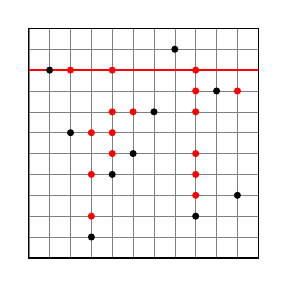
\begin{tikzpicture}[scale=0.265]
        \draw[very thin, gray] (0,0) grid (11,11);
        
        \draw[red, thick] (0,9) -- (11,9);

        \filldraw[black] (3,1) circle (4pt);
        \filldraw[black] (8,2) circle (4pt);
        \filldraw[black] (10,3) circle (4pt);
        \filldraw[black] (4,4) circle (4pt);
        \filldraw[black] (5,5) circle (4pt);
        \filldraw[black] (2,6) circle (4pt);
        \filldraw[black] (6,7) circle (4pt);
        \filldraw[black] (9,8) circle (4pt);
        \filldraw[black] (1,9) circle (4pt);
        \filldraw[black] (7,10) circle (4pt);
        \filldraw[red] (3,2) circle (4pt);
        \filldraw[red] (8,3) circle (4pt);
        \filldraw[red] (3,4) circle (4pt);
        \filldraw[red] (8,4) circle (4pt);
        \filldraw[red] (4,5) circle (4pt);
        \filldraw[red] (8,5) circle (4pt);
        \filldraw[red] (3,6) circle (4pt);
        \filldraw[red] (4,6) circle (4pt);
        \filldraw[red] (4,7) circle (4pt);
        \filldraw[red] (5,7) circle (4pt);
        \filldraw[red] (8,7) circle (4pt);
        \filldraw[red] (8,8) circle (4pt);
        \filldraw[red] (10,8) circle (4pt);
        \filldraw[red] (2,9) circle (4pt);
        \filldraw[red] (4,9) circle (4pt);
        \filldraw[red] (8,9) circle (4pt);
        \draw[black, line width=0.5pt] (0,0) rectangle (11,11); 
    \end{tikzpicture}
    \hfill 
    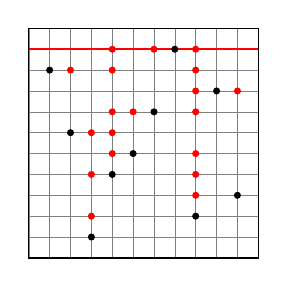
\begin{tikzpicture}[scale=0.265]
        % Desenha o quadriculado
        \draw[very thin, gray] (0,0) grid (11,11);
        
        \draw[red, thick] (0,10) -- (11,10);

        \filldraw[black] (3,1) circle (4pt);
        \filldraw[black] (8,2) circle (4pt);
        \filldraw[black] (10,3) circle (4pt);
        \filldraw[black] (4,4) circle (4pt);
        \filldraw[black] (5,5) circle (4pt);
        \filldraw[black] (2,6) circle (4pt);
        \filldraw[black] (6,7) circle (4pt);
        \filldraw[black] (9,8) circle (4pt);
        \filldraw[black] (1,9) circle (4pt);
        \filldraw[black] (7,10) circle (4pt);
        \filldraw[red] (3,2) circle (4pt);
        \filldraw[red] (8,3) circle (4pt);
        \filldraw[red] (3,4) circle (4pt);
        \filldraw[red] (8,4) circle (4pt);
        \filldraw[red] (4,5) circle (4pt);
        \filldraw[red] (8,5) circle (4pt);
        \filldraw[red] (3,6) circle (4pt);
        \filldraw[red] (4,6) circle (4pt);
        \filldraw[red] (4,7) circle (4pt);
        \filldraw[red] (5,7) circle (4pt);
        \filldraw[red] (8,7) circle (4pt);
        \filldraw[red] (8,8) circle (4pt);
        \filldraw[red] (10,8) circle (4pt);
        \filldraw[red] (2,9) circle (4pt);
        \filldraw[red] (4,9) circle (4pt);
        \filldraw[red] (8,9) circle (4pt);
        \filldraw[red] (4,10) circle (4pt);
        \filldraw[red] (8,10) circle (4pt);
        \filldraw[red] (6,10) circle (4pt);
        \draw[black, line width=0.5pt] (0,0) rectangle (11,11); 
    \end{tikzpicture}
    \caption{Execução do Greedy Future para a sequência X = (3,8,10,4,5,2,6,9,1,7) de acessos.}
\label{fig:GreedyFuture-funcionamento}
\end{figure}

De maneira prática, o algoritmo analisa os pontos de $P'$ na reta horizontal $r$ com $y = i$, com $i \in \{1,\ldots,m\}$ de maneira crescente. Assim, após satisfazer todos os pontos com coordenada $y = i$, sabemos que todos os pares de pontos que estão abaixo ou na reta $r$ estão satisfeitos. Assim, por construção, o resultado do algoritmo é um conjunto arboreamente satisfeito.

O comportamento desse algoritmo é caracterizado por uma abordagem gulosa local. Esse algoritmo quando refletido no contexto de ABBs visita apenas as chaves que estão no caminho da chave buscada e reorganiza todos os nós visitados de maneira a deixar mais perto da raiz, as próximas chaves a serem visitados, e consequentemente, mais longe da raiz as chaves a serem visitados mais tarde. 

Embora o algoritmo garantir encontrar uma solução válida, ou seja um conjunto de pontos $P'$ arboreamente satisfeito, o Greedy Future não garante encontrar minASS. Veja a Figura~\ref{fig:greedy_subotimo}.

\begin{figure}
    \centering
    
    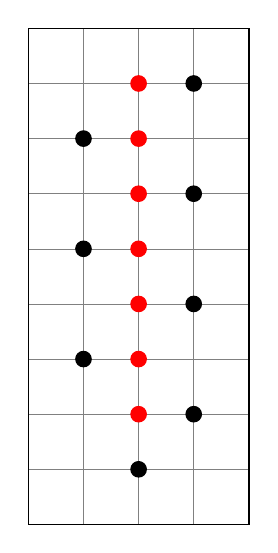
\begin{tikzpicture}[scale=0.7]
        \draw[very thin, gray] (0,0) grid (4,9);

        \filldraw[black] (2,1) circle (4pt);
        \filldraw[black] (3,2) circle (4pt);
        \filldraw[black] (1,3) circle (4pt);
        \filldraw[black] (3,4) circle (4pt);
        \filldraw[black] (1,5) circle (4pt);
        \filldraw[black] (3,6) circle (4pt);
        \filldraw[black] (1,7) circle (4pt);
        \filldraw[black] (3,8) circle (4pt);
        \filldraw[red] (2,2) circle (4pt);
        \filldraw[red] (2,3) circle (4pt);
        \filldraw[red] (2,4) circle (4pt);
        \filldraw[red] (2,5) circle (4pt);
        \filldraw[red] (2,6) circle (4pt);
        \filldraw[red] (2,7) circle (4pt);
        \filldraw[red] (2,8) circle (4pt);
        
        \draw[black, line width=0.5pt] (0,0) rectangle (4,9);
    \end{tikzpicture}
    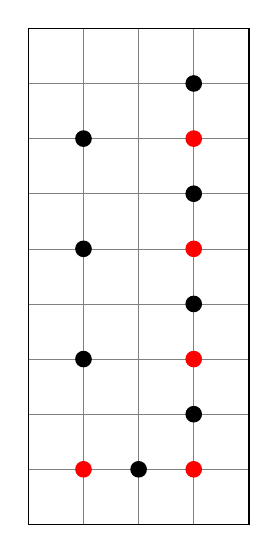
\begin{tikzpicture}[scale=0.7]
        \draw[very thin, gray] (0,0) grid (4,9);
        
        \filldraw[black] (2,1) circle (4pt);
        \filldraw[black] (3,2) circle (4pt);
        \filldraw[black] (1,3) circle (4pt);
        \filldraw[black] (3,4) circle (4pt);
        \filldraw[black] (1,5) circle (4pt);
        \filldraw[black] (3,6) circle (4pt);
        \filldraw[black] (1,7) circle (4pt);
        \filldraw[black] (3,8) circle (4pt);
        \filldraw[red] (1,1) circle (4pt);
        \filldraw[red] (3,1) circle (4pt);
        \filldraw[red] (3,3) circle (4pt);
        \filldraw[red] (3,5) circle (4pt);
        \filldraw[red] (3,7) circle (4pt);
        
        \draw[black, line width=0.5pt] (0,0) rectangle (4,9);
    \end{tikzpicture}
    \caption{Em preto, os pontos dados por uma sequência de acessos. À esquerda, o conjunto de pontos produzidos pelo Greedy Future. À direita, o menor conjunto arboreamente satisfeito para a entrada, de tamanho minASS.}
\label{fig:greedy_subotimo}
\end{figure}

